
%!TEX program = xelatex
\documentclass[letterpaper,12pt]{exam}
\usepackage{../videoNotes}
\usepackage{xcolor}
\usepackage[dvipsnames]{xcolor}
\usepackage{soul}

\newcommand{\unit}{Unit 02}
\pagestyle{headandfoot}
\firstpageheader{CSC 264 \semester\ \  \unit}{}{Name: $\rule{6cm}{0.15mm}$}
\runningheader{CSC 264 \semester}{\unit}{Page \thepage\ of \numpages}
\firstpagefooter{}{}{}
\runningfooter{}{}{}

\begin{document}



\section*{\unit\_010 -- Debugging, Registers, and Arithmetic} 
\par{\fontfamily{qzc}\selectfont\textbf{Video Length 9:15 }}
\begin{questions}

\begin{samepage}
    \question What program will we be using for terminal debugging?
    \vspace{5mm}
\end{samepage}
\par
 \begin{samepage}
     \question What program can we use for graphical debugging?
     \vspace{5mm}
 \end{samepage}
 \par
  
 \section*{\unit\_020 -- Debugging with GDB }
 \par{\fontfamily{qzc}\selectfont\textbf{Video Length 4:30}}
 \begin{samepage}
     \question Why are extra labels useful for debugging?
     \vspace{5mm}
 \end{samepage}
 \begin{samepage}
     \question What flag must be added to allow assembly programs to be loaded into the gdb debugger?
     \vspace{5mm}
 \end{samepage}
 \par
  \begin{samepage}
      \question What gdb command would be used to set a breakpoint at the \_exit label?  (You may do it with or without the asterisk)
      \vspace{5mm}
  \end{samepage}
  \par
   \begin{samepage}
       \question What gdb command is used to run the program?
       \vspace{5mm}
   \end{samepage}
   \par
    \begin{samepage}
        \question What gdb command is used to step through the next statement?
        \vspace{5mm}
    \end{samepage}
    \par
     \begin{samepage}
         \question What gbd command is used to print the contents of the rax register in decimal? \rule{5cm}{0.15mm}
         \vspace{5mm}
         \question What gbd command is used to print the contents of the rax register in hexadecimal? \rule{5cm}{0.15mm}
         \vspace{5mm}
         \question What gbd command is used to print the contents of the rax register in binary? \rule{5cm}{0.15mm}
         \vspace{5mm}
         \question What gbd command is used to print the contents of the rax register as an ASCII character? \rule{5cm}{0.15mm} (Note, I did not do it in the video, the format specifier is "c")
         \vspace{5mm}

        \end{samepage}
     \par

     \begin{samepage}
         \question What gdb command would be used to print the contents of the sum label in hex.  The value is stored in 1 byte. \rule{5cm}{0.15mm}
         \vspace{5mm}
     \end{samepage}
     \par
     \begin{samepage}
         \question What gdb command would be used to print the contents of the sum label in hex.  The value is stored in 2 bytes. \rule{5cm}{0.15mm}
         \vspace{5mm}
     \end{samepage}
     \par
     \begin{samepage}
         \question What gdb command would be used to print the contents of the sum label in hex.  The value is stored in 4 bytes. \rule{5cm}{0.15mm}
         \vspace{5mm}
     \end{samepage}
     \par
     \begin{samepage}
         \question What gdb command would be used to print the contents of the sum label in hex.  The value is stored in 8 bytes. \rule{5cm}{0.15mm}
         \vspace{5mm}
     \end{samepage}
     \par
      
     \begin{samepage}
         \question What gdb command would be used to print all of the registers?
         \vspace{5mm}
     \end{samepage}
     \par
      \section*{\unit\_020 gdb part 2 -- }
      \par{\fontfamily{qzc}\selectfont\textbf{Video Length }}
      \begin{samepage}
          \question What question do you use to exit from gdb?
          \vspace{5mm}
      \end{samepage}
    
      \rule{0.5\textwidth}{.4pt} %End of section
      %----------------------------------
      
 \rule{0.5\textwidth}{.4pt} %End of section
 %----------------------------------
\section*{\unit\_030 -- debugging with kdbg}
\par{\fontfamily{qzc}\selectfont\textbf{Video Length 11:45}}
\begin{samepage}
    \question Please try to run kdbg on your machine.  Try to install it if you do not have it.  Did it work?  If you did get it to work, what did you have to do to get it working?
    \vspace{55mm}
\end{samepage}

\rule{0.5\textwidth}{.4pt} %End of section

\section*{\unit\_040 -- Register Recap}
\par{\fontfamily{qzc}\selectfont\textbf{Video Length }}
\begin{samepage}
    \question Why are registers faster than memory?
    \vspace{5mm}
\end{samepage}

\begin{samepage}
    \question Are "General Purpose Registers" really general purpose? Explain your answer.
    \vspace{5mm}
\end{samepage}
\par
 

\rule{0.5\textwidth}{.4pt} %End of section
%----------------------------------
\section*{\unit\_050 -- Registers}
\par{\fontfamily{qzc}\selectfont\textbf{Video Length }}
\begin{samepage}
    \question  What does GPR mean? 
    \vspace{5mm}
\end{samepage}
\begin{samepage}
    \question Which register is used as an accumulator for arithmetic operations and for return values from functions?
    \vspace{5mm}
\end{samepage}
\begin{samepage}
    \question Which register is used as a base pointer?
    \vspace{5mm}
\end{samepage}
\begin{samepage}
    \question Which register is used as a loop counter?
    \vspace{5mm}
\end{samepage}
\begin{samepage}
    \question Which register is used an an I/O pointer and in multiplication and divsion?
    \vspace{5mm}
\end{samepage}
\par
Note: We are going to ignore the RSP and the RBP registers for now.
\par
\begin{samepage}
    \question What eight GPRs were added to 64-bit systems?
    \vspace{5mm}
\end{samepage}
\par
\begin{samepage}
    \question What is the name of the Instruction Pointer? on 64-bit systems?
    \vspace{5mm}
\end{samepage}
\par
\begin{samepage}
    \question What is the name of the register that hold the flags on 64-bit systems?
    \vspace{5mm}
\end{samepage}
\par
\section*{\unit\_060 -- Register Sizes }
\par{\fontfamily{qzc}\selectfont\textbf{Video Length 4:30}}
\begin{samepage}
    \question How are register sizes specified in x86 Assembler?
    \vspace{5mm}
\end{samepage}
\begin{samepage}
    \question What prefix was used for 16 bit registers on 8086 processors? (Warning: Trick question)
    \vspace{5mm}
\end{samepage}

\begin{samepage}
    \question What prefix is used when referring to 32-bit registers?
    \vspace{5mm}
\end{samepage}
\par
\begin{samepage}
    \question What prefix is used when referring to 64-bit registers?
    \vspace{5mm}
\end{samepage}
\par
\begin{samepage}
    \question What prefix would be used to refer to the entire 64 bits of the R12 register?
    \vspace{5mm}
\end{samepage}
\par
\begin{samepage}
    \question What prefix would be used to refer to the lower 32 bits of the R12 register?
    \vspace{5mm}
\end{samepage}
\par
    \begin{samepage}
        \question What prefix would be used to refer to the lower 16 bits of the R12 register?
        \vspace{5mm}
    \end{samepage}
    \par
\begin{samepage}
    \question What prefix would be used to refer to the lower 8 bits of the R12 register?
    \vspace{5mm}
\end{samepage}
\par
      
    \rule{0.5\textwidth}{.4pt} %End of section
\section*{\unit\_065 -- Moving LSB }
\par{\fontfamily{qzc}\selectfont\textbf{Video Length 13:00}}
\begin{samepage}
    \question What does LSB stand for?
    \vspace{5mm}
\end{samepage}
\par
 
\begin{samepage}
    \question Assume that the RAX register contains a 64-bit value.  What assembly language instruction would move the Least Significant 32 bits of the RAX to the RBX register?
    \vspace{5mm}
\end{samepage}
\begin{samepage}
    \question In the video I was showed a preference for hex over decimal.  Why is that?
    \vspace{35mm}
\end{samepage}
\par
\section*{\unit\_075 -- mov Program}
\par{\fontfamily{qzc}\selectfont\textbf{Video Length }}
\par 
note: I am asking only one question about each of the three parts of the program.  However, \textbf{\textit{you should know how each of the lines works, even if there is no question about it.}}
\par 
\begin{samepage}
    \question Write the code needed for the .data section to declare memory labeled "widget" that will hold 32 bits and is initialized to 0.
    \vspace{5mm}
\end{samepage}
\begin{samepage}
    \question Write the code that would move the LSB 16 bits of rbx register into the LSB 16 bits of the r8 register.
    \vspace{5mm}
\end{samepage}
\par
 \begin{samepage}
     \question What system call that would move the 32 LSB of the R8 register into the widget memory location ?
     \vspace{5mm}
 \end{samepage}
 \par
  
%----------------------------------
  %%%%%%%%%%%%%%%%%%%%%%%%%%%%%%%%%%%%%%%%%%%%%%%%%%%%%
\begin{center}
    \rule{0.5\textwidth}{.4pt}
\end{center}
Do you have any questions or concerns? Please write any lingering questions you have here.

%----------------------------------
\end{questions}
%footer
\vfill
\begin{center}
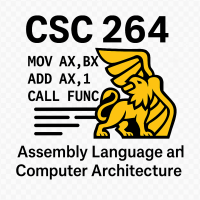
\includegraphics{../csc264Logo}
\end{center}
\end{document} 